%Auteure : Eloïse Rotondo

\subsubsection{Fonctionnement}

Comme son nom l’indique, un \textit{\gls{blockchain} bridge} également appelé \textit{\gls{cross-chain} bridge} est un protocole reliant deux \textit{\gls{blockchain}s} entre elles de manière unilatérale ou bilatérale dans une optique d’interopérabilité.\\

Dans la but de comprendre la popularité des \textit{bridges} en tant que protocole d’interopéralité, il faut en premier lieu s’intéresser au marché de la cryptomonnaie. Actuellement \gls{Bitcoin} domine en représentant 40,5\% de ce dernier, suivie ensuite par \gls{Ethereum} avec 19,5\%. Cela laisse donc 40\% du marché formé de nombreuses crytomonnaies plus petites et plus indépendantes. C’est donc naturellement, qu’une forte demande de possibilité d’échanges entre les \textit{\gls{blockchain}s} ait vu le jour de la part des utilisateurs ayant plusieurs cryptomonnaies\cite{NgraveNumbers}.\\

Il existe trois différentes manières de déplacer les \gls{actif}s en tant que \textit{bridge}. Tout d’abord, le mécanisme de \textit{Lock and Mint} signifiant Verrouiller et Frapper, les \gls{actif}s se trouvant sur la chaîne de départ sont verrouillés sur celle-ci pour être ensuite créés sur la chaîne destinataire. Un autre mode d'échange est celui du \textit{Burnt and Mint}, ce dernier est très similaire à celui déjà présenté, la seule différence étant que les \gls{actif}s sont directement effacés plutôt que verrouillés. Pour finir, les échanges atomiques entre chaînes (Atomic Swaps) permettent un échange direct en pair-à-pair d'\gls{actif}s entre la chaîne d’origine et la chaîne de destinataire.\cite{EthereumMechanism}

\subsubsection{Mécanisme de vérification}

Comme évoqué précédemment, deux \textit{\gls{blockchain}s} ne peuvent pas communiquer directement entre elles, par conséquent lors de l’utilisation d’un \textit{bridge} les deux chaînes ne se connaissent pas et ont seulement connaissance des évènements se produisant sur leur chaîne respectives. Il est donc nécessaire d’établir une relation de confiance entre les deux chaînes pour qu’elles puissent accepter de communiquer. Pour cela, les \textit{bridges} emploient un mécanisme utilisant des vérificateurs. Un vérificateur est une entité connectée en tant que noeud au réseau de la \textit{blockchain}. Ce dernier agit comme autorité de confiance, vérifiant et validant les transactions sur cette dernière. Un noeud d'une \textit{blockchain} est un ordinateur connecté au réseau de cette dernière. Un \textit{client} est un logiciel permettant de transformer un ordinateur en noeud. \cite{EthereumNodeClient} \\


Il existe un grand nombre de \textit{bridges}, chacun avec leurs propres spécificités mais ils peuvent généralement être séparés en deux catégories les \textit{Trusted \gls{blockchain} Bridge} et les \textit{Trustless \gls{blockchain} Bridge}. \\


Les \textit{Trusted Bridges} sont vérifiés de manière externe car ils utilisent un ensemble de vérificateurs tiers pour transmettre des données entre les chaînes. Ils ont pour avantage leur rapidité, leur moindre coût et la facilité d'échange avec tous les types de données acceptés par les \textit{\gls{blockchain}s}. Cependant les vérificateurs externes sont moins fiables que ceux de la chaîne.\cite{EthereumBridges}

Les \textit{Trustless Bridges} sont désignés comme \textit{trustless} car ils dépendent des chaînes dont ils font l’intermédiaire pour transférer des données ou des \gls{actif}s. Par conséquent leur niveau de fiabilité est égal à celui des \textit{\gls{blockchain}s} et il n’est pas nécessaire de faire confiance à un ensemble de vérificateurs tiers (contrairement aux autres \textit{bridges}). Pour cette raison, ils sont reconnus comme étant plus fiables que les \textit{trusted bridges}.\cite{EthereumBridges}\\


 Les \textit{bridges} peuvent également être distingués en fonction de leur type de vérification. Les plus connus sont la vérification native, externe et locale.\cite{InteroperabilityBhuptani} \\

La vérification native commence par l’utilisation d’un noeud léger. \cite{NomadDocsNative} Un noeud léger aussi connu sous le nom de client léger est un logiciel permettant de connecter les noeuds des \textit{\gls{blockchain}s} entre elles. Il est codé comme un \textit{\gls{smart contract}} puis est employé de la chaîne de l'expéditeur vers la machine virtuelle de la chaîne destinataire. Si les vérificateurs de données de la chaîne de l'expéditeur agissent de manière correcte alors le noeud léger est vu comme véridique par la chaîne réceptionnant les \gls{actif}s ou données et peut être utilisé de manière bilatérale.
 Un avantage de cette solution est qu’elle est reconnue comme étant celle reposant le moins sur la confiance parmi celles existantes car les chaînes ne se fient qu’à leurs propres vérificateurs pour effectuer le \textit{bridge}. Un autre bénéfice de ce mécanisme est le fait qu’il n’utilise pas de vérificateurs tiers entre les deux \textit{\gls{blockchain}s} et donc la sécuté du réseau dépend des \textit{\gls{blockchain}s} elles-même (ce qui est avantageux car elles sont robutes et préparées aux attaques comme la chaîne d’Ethereum par exemple).
 Un désavantage de cette méthode est que le noeud léger doit être adapté aux consensus des chaînes auquelles il est attaché ce qui le rend inutilisable avec des chaînes différentes. Le noeud léger nécessite également de la maintenance en cas de changement des règles consensus (utilisées pour valider les transactions). Un autre inconvénient découlant du fait que le noeud léger est programmé de manière spécifique est que ce dernier n’est donc pas réutilisable. \\

\pagebreak

La vérification externe consiste en un ensemble de vérificateurs n’appartenant pas aux \textit{\gls{blockchain}s} relayant les données entre les deux extrémités du \textit{bridge}. Pour se faire, un certains nombre de vérificateurs doivent signer un message provenant de la chaîne d’envoi pour que le chaîne destinataire le reconnaisse comme valide. Par exemple, pour le \textit{bridge} \gls{Wormhole} 13 vérificateurs sur 19 doivent avoir signé\cite{NomadDocsExternal}. Ce concept est une primitive cryptographique (algorithme cryptographique de bas niveau servant de base à un système de sécurité informatique) nommée le système de signature à seuil (désignée par TSS pour \textit{Threshold Signature Scheme})\cite{BinanceTSS}. 
Contrairement à la vérifications native, les \textit{bridges} vérifiés de manière externe sont faciles à développer, peuvent être réutilisés sans problèmes et leur maintenance coûte peu. Le désavantage conséquent de cette méthode est que la sécurité dépend des vérificateurs tiers du pont ce qui peut fragiliser le système car ils sont généralement moins sécurisés que ceux des \textit{\gls{blockchain}s}. \\


\begin{figure}[h!]
    \centering
\stackunder{
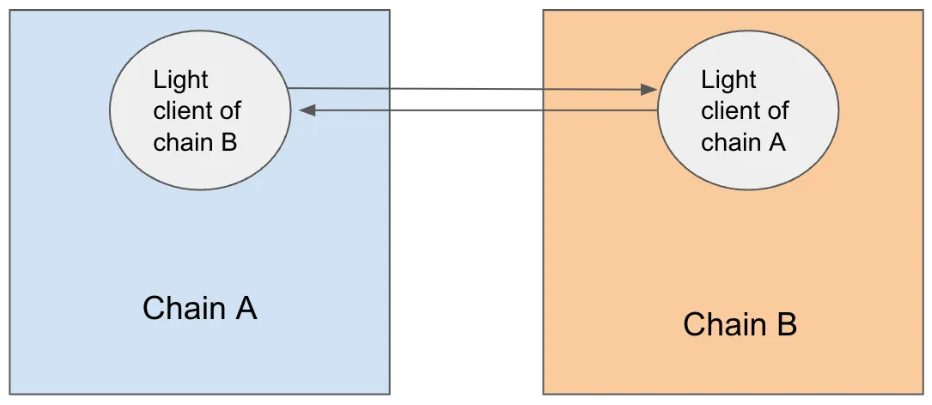
\includegraphics[scale=0.60]{centralisation/imagesBridges/LightClient.png}}
    {\scriptsize
            Source: \url{https://docs.nomad.xyz/the-nomad-protocol/verification-mechanisms/native-verification}}
    \caption{Mécanisme utilisant un noeud léger.}
    \label{fig:LightClient}
\end{figure}

\pagebreak

La vérification externe consiste en un ensemble de vérificateurs n’appartenant pas aux \textit{\gls{blockchain}s} relayant les données entre les deux extrémités du \textit{bridge}. Pour se faire, un certains nombre de vérificateurs doivent signer un message provenant de la chaîne d’envoi pour que le chaîne destinataire le reconnaisse comme valide. Par exemple, pour le \textit{bridge} Wormhole 13 vérificateurs sur 19 doivent avoir signé\cite{NomadDocsExternal}. Ce concept est une primitive cryptographique (algorithme cryptographique de bas niveau servant de base à un système de sécurité informatique) nommée le système de signature à seuil (désignée par TSS pour \textit{Threshold Signature Scheme})\cite{BinanceTSS}. 
Contrairement à la vérifications native, les \textit{bridges} vérifiés de manière externe sont faciles à développer, peuvent être réutilisés sans problèmes et leur maintenance coûte peu. Le désavantage conséquent de cette méthode est que le bon fonctionnement du système dépend des vérificateurs tiers ce qui peut le fragiliser car ils sont généralement moins fiables que ceux des \textit{\gls{blockchain}s}. \\

Il est intéressant de noter que les \textit{\gls{blockchain}s} ont également leur propre ensemble de vérificateurs sous la forme de vérificateur de données. Ces derniers sont utilisés lors de la vérification locale. Lors de la vérification locale, les chaînes se vérifient entre elles en utilisant un vérificateur en tant que représentant.

\begin{figure}[h]
    \centering
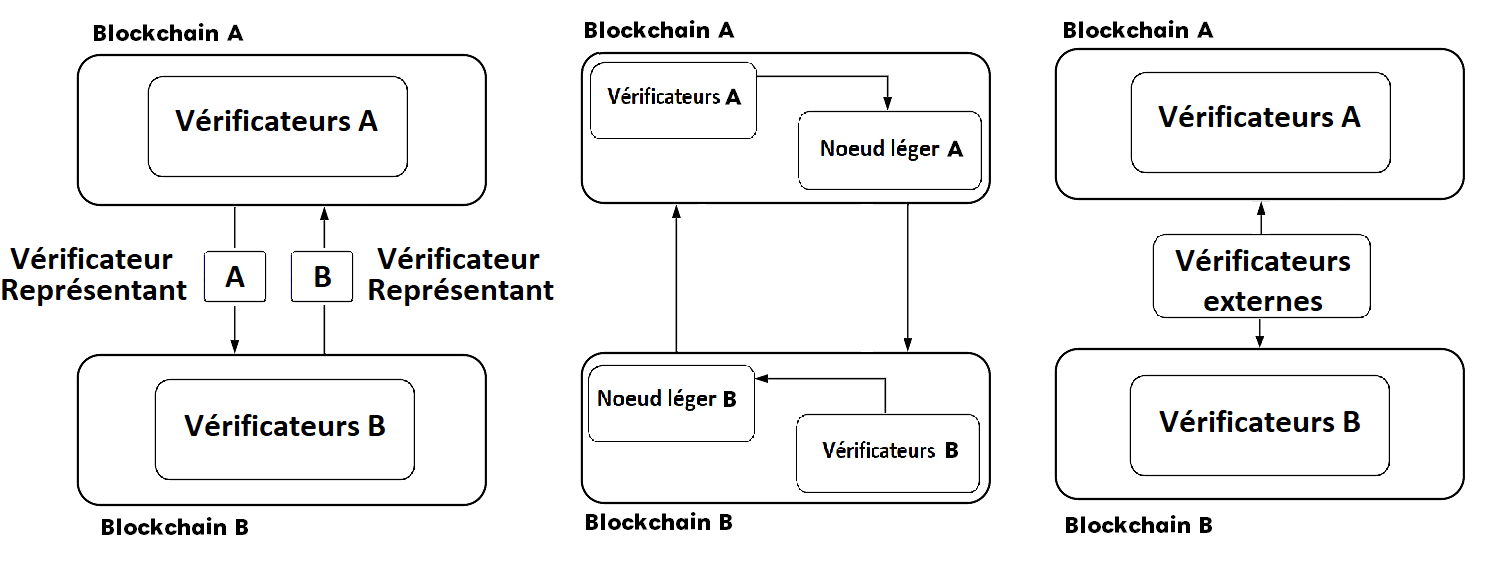
\includegraphics[scale=0.60]{centralisation/imagesBridges/DiagrammeResumeVerif.png}
\caption{Résumé des types de vérification. (locale, native et externe)}
\label{fig:LocaleVerif}
\end{figure}

\subsubsection{Les risques liés aux Bridges}

La popularité des \textit{\gls{blockchain} Bridges} pour les échanges centralisés ne cesse d’augmenter au fils du temps mais il est important de comprendre que comme tout outil, ces derniers ne sont pas sans risques. \\

Les \textit{bridges trustless} utilisent des \textit{\gls{smart contract}s} lors du processus d’échange dans le but de le rendre autonome afin de ne pas utiliser une entité centrale entre les deux \gls{blockchain}s. Cependant ces \textit{bridges} sont néanmoins centralisés car ils utilisent les vérificateurs pour obtenir un consensus lors des transactions.
Un \textit{\gls{smart contract}} étant un script écrit par un développeur, il est possible que certaines erreurs puissent s’être glissées dans le code par inadvertance ou bien qu’il existe des failles dans le programme permettant aux attaquants de le détourner pour un profit personnel. 
Pour minimiser ce type de risques, il est recommandé d’effectuer des audits sur les \textit{bridges.} \\

Une faiblesse spécifique des \textit{bridges trusted} repose sur le fait que les utilisateurs doivent léguer le contrôle de leurs \gls{actif}s et faire confiance aux vérificateurs externes aux \gls{blockchain}s. Sauf que dans certains cas, ces derniers peuvent coopérer pour tromper les utilisateurs en récupérant leurs \gls{actif}s puis en disparaissant comme dans les \textit{rug pull}\cite{EthereumRisks}. Ce modèle d’escroquerie peut être scindé en deux catégorie : les \textit{hard rug pull} et les \textit{soft rug pull}\cite{Hacken}. Le premier cas est basé sur un piège présent dans le code d’un \textit{\gls{smart contract}} empêchant les utilisateurs d’utiliser ou revendre les \gls{actif}s frappés, seul le fraudeur en a le droit. Il peut donc en toute tranquillité revendre les \gls{actif}s et récupérer l’argent. En revanche, pour les \textit{soft rug pull}, les utilisateurs ne sont pas coincés avec des \gls{actif}s verrouillés mais les fraudeurs utilisent des techniques psychologiques. En effet, les escrocs rendent attirant leur projet pour que les clients investissent et hésitent à se retirer par peur de perdre leur investissent (souvent de taille conséquent) puis les créateurs de la fraude disparaissent avec leurs \gls{actif}s.\\

Comme vu dans la section présentant les différentes méthodes d’échange des \textit{bridges}, ces derniers frappent les \gls{actif}s désirés sur la chaîne destinataire. Certains attaquants peuvent profiter de ce mécanisme de frappe pour effectuer ce qu’on appelle une \textit{Infinite Mint Attack}.\cite{ChainLinkRisks} Cette attaque peut se résumer à un \textit{hacker} générant un nombre élevé d’\gls{actif}s en utilisant une faille d’un \textit{bridge} sans verrouiller ou brûler d’\gls{actif}s sur sa \textit{\gls{blockchain}}. Suite à cela, l’individu réintroduit ces \gls{actif}s sur le marché ce qui fait violemment baisser leur coût ce qui engendre un risque financier systémique.\\

Les \textit{\gls{blockchain} Bridges} sont devenus un outil indispensable des échanges centralisés très rapidement, mais il ne faut pas oublier que ces protocoles sont relativement récents. Créés par de petites \gls{blockchain}s comme Syscoin et NEAR Protocol dans le but de rentre leurs chaînes interopérables avec les applications décentralisées d’\gls{Ethereum}, les premiers bridges datent de 2020\cite{Bitstamp}. Par conséquent, nous ne connaissons pas encore le comportement des \textit{bridges} lorsqu’ils font face à des scénarios sortants de la norme comme des attaques réseaux, un retour en arrière sur les transactions d’une \gls{blockchain} (souvent désigné par le terme \textit{rollback}) ou bien pendant une congestion du réseau. Ces zones d’incertitudes peuvent donc être une source de risques. \\

\begin{figure}[h!]
    \centering
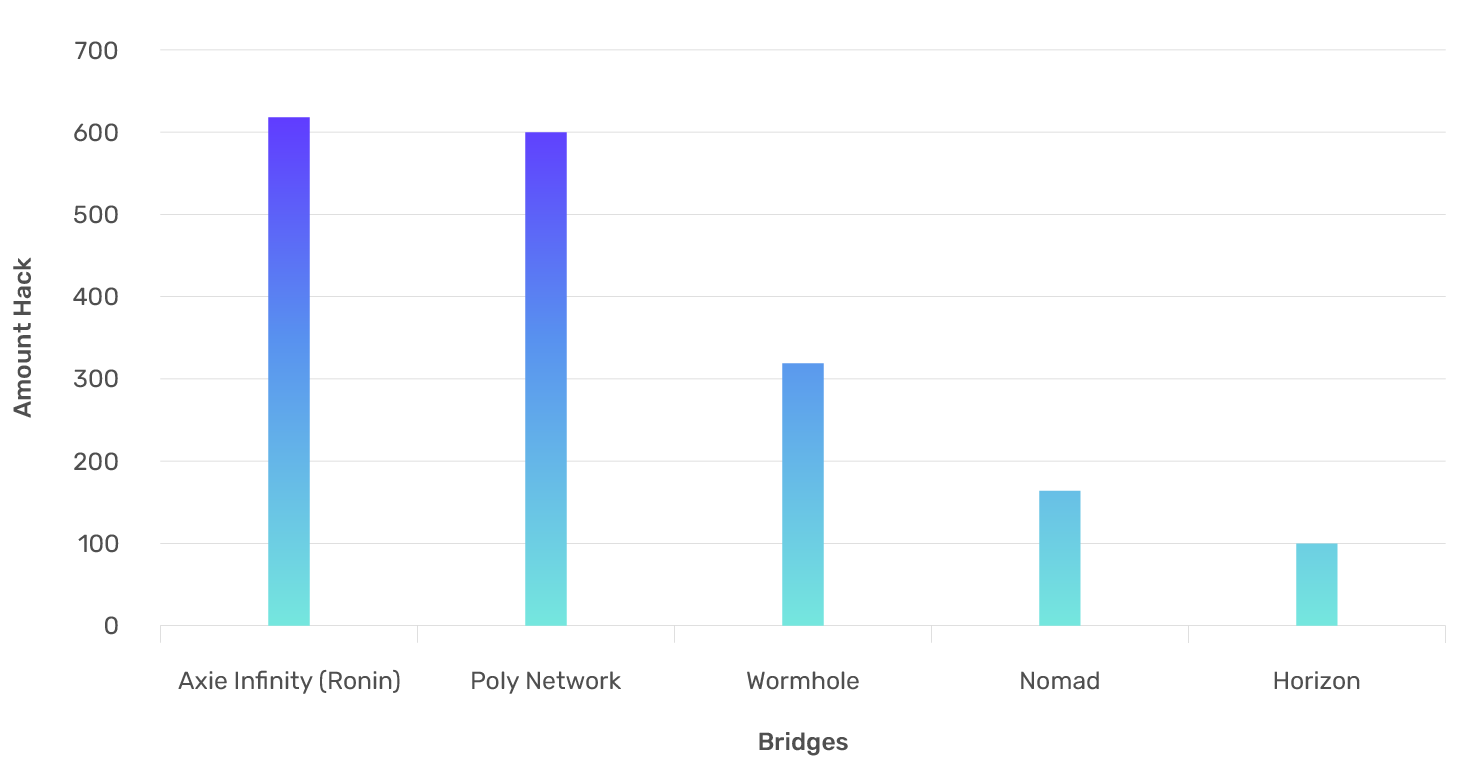
\includegraphics[scale=0.30]{centralisation/imagesBridges/GraphLossesBridges.png}
    {\scriptsize
            Source: \url{https://www.treehouse.finance/insights/blockchain-and-interoperability-globalization-3-0}}
    \caption{Pertes en millions de dollars des bridges les plus connus.}
    \label{fig:GraphBridges}
\end{figure}

\subsection{Le trilemme de l’interopérabilité}

Malgré l’existence de plus d’une centaine de \textit{bridges} différents, les développeurs et les utilisateurs voulant utiliser un \textit{bridge} doivent faire des concessions lors de leur choix vis-à-vis des trois notions de \textit{trustless}, d’extensibilité (\textit{extensible}) et de généralisation (\textit{generalizable}).\\

Le mot trustless peut être traduit par «sans confiance». Si un \textit{bridge} est caractérisé comme \textit{trustless}, cela signifie que celui-ci possède un niveau équivalent à celui d’une ou des chaînes sous-jacentes, il est donc pas nécessaire de faire confiance à une entité externe aux \textit{blockchains}.  La notion  d’extensibilité signifie que le \textit{bridge} est compatible un grand nombre de chaînes.
Un \textit{bridge} respecte la notion de généralisation s’il est capable d'échanger n’importe quel type de données accepté par les deux chaînes.\\

Pour illustrer ces termes, il est possible de les appliquer aux types de vérification appartenant aux \textit{bridges}. La vérification locale respecte les notions d’extensibilité et de \textit{trustless} puisque qu'elle est applicable sur tous les \textit{bridges} peu importe les chaînes reliées et le niveau de fiabilité dépend de la chaîne la plus faible.
La vérification native ne respecte pas la notion d’extensibilité car le \textit{bridge} n’est pas réutilisable. Néanmoins elle respecte la notion de généralisation parce qu’elle est codée de manière spécifique aux \textit{\gls{blockchain}s} reliées au \textit{bridge}. Le critère basé sur la notion \textit{trustless} est également rempli étant donné que le niveau de fiabilité dépend des vérificateurs des chaînes.
La vérification externe ne respecte pas la notion de \textit{trustless} cependant elle est fortement extensible et générale vis-à-vis des données. \cite{Ngrave}

 Suite au paragraphe précédent, il est possible de constater que les \textit{bridges} interopérables ne respectent que deux des trois notions énoncées. Ce problème est connu sous le nom de trilemme de l’interopérabilité. 

\subsubsection{Une solution optimiste}

Une solution proposée pour résoudre ce trilemme est un \textit{optimistic bridge}(\textit{bridge} optimiste) nommé vis-à-vis de sa vérification portant le même nom\cite{OptimisticBhuptani}. En effet, contrairement aux \textit{bridges} vérifiés de manière native, locale ou externe, la vérification optimiste dépend de l’utilisation d’une latence lors de la confirmation du transfert des \gls{actif}s entre les \textit{\gls{blockchain}s}. Cela priorise donc la sécurité au détriment de la vivacité, puisque les transactions sont par conséquent plus lentes mais sécurisées car le \textit{bridge} est \textit{trustless}. \\

Voici plus en détails le déroulement du processus de vérification optimiste d’un \textit{bridge}.
Ceci commence par l’envoi d'une demande de transaction de la part d’un utilisateur ou d’une application décentralisée vers la \textit{\gls{blockchain}} native par le biais d’une fonction contrat. Cette demande est ensuite acceptée par un validateur (une entité équivalente à un vérificateur, la seule différence étant leur rôle) puis inscrite sur un \textit{block} de la chaîne.\cite{NomadDocsVerification}
Ensuite un vérificateur a pour rôle de vérifier la transaction. Pour cela, le vérificateur signe le haché des données envoyées précédemment. 
Suite à cela, n’importe quel système de relais peut lire le haché signé sur la chaîne originelle et l’inscrire sur une ou plusieurs chaînes destinataire. Les validateurs de la chaîne destinataire valide et l'inscrivent sur leur chaîne. Cette action déclenche alors une latence de trente minutes pendant laquelle un observateur peut signaler et prouver une fraude effectuée par la chaîne native ce qui déconnectera la communication avec la chaîne destinataire. 

Deux scénarios sont alors possibles. Premier cas, si aucun observateur ne se manifeste, les données de la transaction sont finalisées puis traitées par la chaîne destinataire. Les validateurs sont récompensés pour leur travail avec une partie des frais de transaction. \cite{Fees} Deuxième cas, un observateur prouve une fraude pendant les trente minutes accordées. Le vérificateur ayant fraudé est pénalisé par la perte de sa récompense (qui sera obtenu par l'observateur) et son exclusion du réseau.\cite{EthereumSlashing}

\subsubsection{Possibles faiblesses de l’optimisme et leurs solutions}

Le bon fonctionnement des \textit{bridges} optimistes dépend des chaînes auquelles il est rattaché donc tant que ces dernières sont protégées correctement la seule conséquence d’une faille du \textit{bridge} est l’arrêt système plutôt qu’une perte de fonds comme cela peut être le cas avec les autres types de \textit{bridge}.

Les deux acteurs principaux ayant les moyens de nuire au bon fonctionnement du \textit{bridge} ainsi que de la transaction est l’agent vérificateur ainsi que l’observateur car ces deux rôles ont de l’influence sur cette dernière. \\

Le premier cas impliquant le vérificateur se nommant \textit{Updater Fraud} (fraude du vérificateur)  fut déjà mentionné lors de la présentation du fonctionnement du \textit{bridge} optimiste. Ce dernier repose sur le fait que toute transaction doit passer par le vérificateur et que par conséquent toute fraude est originaire de ce dernier. Sinon si cela venait d’un autre participant, le vérificateur n’aurait alors pas accepté la transaction. C’est pourquoi, lors de l’intervention d’un observateur prouvant une fraude, le vérificateur est sanctionné par le retrait sur son solde d'un montant équivalent à la récompense promise et par son exclusion du réseau de la \textit{blockchain}. \\

La seconde faiblesse liée aux vérificateurs est un \textit{Updater DoS} ou déni de services de la part du vérificateur. En effet, il est possible que le processus soit interrompu si un validateur arrête de signer empêchant l'échange inter-chaînes de se produire.
Une solution a été implémentée pour palier à cela comme la mise en place d’un système de substitution avec la présence de plusieurs vérificateurs sur une même chaîne afin de pouvoir prendre le relai en cas de manque de réponse de la part de celui étant rattaché au transfert.  Pour éviter que ce scénario se produise fréquemment le vérificateur ayant manqué son tour lors de la signature (que cela soit accidentel ou voulu) est pénalisé de la même manière que le cas précédent. \\

Maintenant que les possibles obstacles au bon fonctionnement du \textit{bridge} liés au vérificateur ont été mis en lumière, il est également possible que l’observateur ait un comportement malveillant.  Effectivement, malgré l’absence de tromperie (puisque le vérificateur remplit son rôle), l’observateur peut abuser du mécanisme de déclaration de fraude pour impacter le bon déroulement du procédé. \\

La faculté de l’observateur à pouvoir couper la connexion s’il conteste la transaction lui permet d’effectuer un déni de service appelé \textit{Watcher DoS}. C’est pourquoi il lui ait possible de fermer définitivement la connexion d’une transaction si ce dernier continue sans cesse de couper le processus sans raison valable. Heureusement, la fermeture ne concerne que la connexion et n’impacte en aucun cas le système du \textit{bridge}. Cependant cette attaque semble irrationnelle en terme de ressources et de temps car l’observateur effectuant le déni de service ne gagne rien financièrement contrairement au processus habituel. En effet, si un observateur prouve une fraude correctement, ce dernier peut récupérer la récompense du vérificateur. Mais ici puisqu’aucune fraude n’est prouvée les données se trouvant sur la chaîne d’origine sont conservées et sécurisés. Cela cause seulement une perte de temps pour l’utilisateur ou l’application décentralisée voulant effectuer l'échange d’une \textit{\gls{blockchain}} à une autre.

Une réponse à ce problème actuellement mise en œuvre par le \textit{bridge} de \gls{Nomad} est la présence d’un groupe restreint d’observateurs autorisés à contester, de cette manière il est facile de connaître les observateurs malveillants. Chaque observateur possède une clé permettant de signer une attestation confirmant la présence d’une fraude dans la transaction, chaque \textit{bridge} stocke un ensemble contenant les adresses des attestations appartenant aux observateurs autorisés. Si l’attestation reçue par le \textit{bridge} est présente dans l’ensemble alors la connexion est rompue\cite{NomadDocsWatcher}.
Sur le long terme, une proposition consistant à la mise en place de frais si l’on souhaite contester est en train d’être étudiée. Le montant doit répondre à deux contraintes: ce dernier doit être assez haut pour dissuader les observateurs malhonnêtes mais assez bas pour que ceux ayant réellement l’envie de prouver de manière valide une fraude existante puissent le faire. Dans la continuité de cette solution, il serait également possible de récupérer la signature de la déconnexion générée par l’observateur sur la chaîne originale et de le pénaliser en lui retirant les frais qu’il a payé tel une garantie\cite{OptimisticBhuptani}.

